\documentclass[letterpaper, 10 pt, conference]{ieeeconf}
\IEEEoverridecommandlockouts
\overrideIEEEmargins
\let\proof\relax
\let\endproof\relax
\usepackage{amsmath,amssymb,amsfonts}
\usepackage{amsthm}
\usepackage{algorithmic}
\usepackage{algorithm}
\usepackage{graphicx}
\usepackage{graphbox}
\usepackage{textcomp}
\usepackage{multirow}
\usepackage{xcolor}
\usepackage[export]{adjustbox}
\usepackage{color}
\def\BibTeX{{\rm B\kern-.05em{\sc i\kern-.025em b}\kern-.08em
    T\kern-.1667em\lower.7ex\hbox{E}\kern-.125emX}}
    
\setlength{\tabcolsep}{0.4em}


%%%%% PARA LINKAR REFSSSSS %%%%%
\makeatletter
\let\NAT@parse\undefined
\makeatother
\usepackage{hyperref}
%%%%%%%%%%%%%%%%%%%%%%%%%%%%%%%%

\title{\LARGE\bf AROB Practical Work}


\author{\centering Author 1, Author 2}

\begin{document}
\maketitle


\begin{abstract}

Practical work abstract. 200 words approx.

\end{abstract}

%%%%%%%%%%%%%%%%           
% INTRODUCTION %
%%%%%%%%%%%%%%%%

\section{Introduction}\label{sec:intro}
Small introduction to motivate the algorithm and relevant bibliography.
This is an example to add a citation in Latex~\cite{thrun2005probabilistic}.

%%%%%%%%%%%%%%%%%%%           
%% PRELIMINARIES %%
%%%%%%%%%%%%%%%%%%%

\section{Algorithm description}\label{sec:algorithm}
Short description of the algorithm.

This is an example to include an equation in the document,
\begin{equation}
\label{Eq:eq1}
    \dot{x} = v \cos(\theta).
\end{equation}
Equation~\eqref{Eq:eq1} shows part of the kinematics of a unicycle vehicle.


%%%%%%%%%%%%%%%%%%%%%%%%           
%%% IMPLICIT CONTROL %%%
%%%%%%%%%%%%%%%%%%%%%%%%

\section{Implementation details}\label{sec:implementation}
Relevant details of your implementation. You can include a pseudo-code algorithm, like the one in Algorithm~\ref{alg:alg1}.
\renewcommand{\algorithmiccomment}[1]{{\small// \textit{#1.}}}
\begin{algorithm}[!ht]
\caption{Pseudo-RRT}
\label{alg:alg1}
\begin{algorithmic}[1]
\REQUIRE $x_0$ and $x_g$
\STATE Initialize Tree with $x_0$
\WHILE{$x_g$ not reached}
    \STATE $x_r =$ Generate a random location
    \STATE $x_n =$ Nearest(Tree,$x_r$)
    \IF{ObstacleFree$(x_r,x_n)$}
        \STATE Add $x_r$ to Tree
        \STATE Check if $x_g$ is reachable from $x_r$
    \ENDIF
\ENDWHILE
\RETURN Path from $x_0$ to $x_g$
\end{algorithmic}
\end{algorithm}


%%%%%%%%%%%%%%           
%% EXAMPLES %%
%%%%%%%%%%%%%%

\section{Experimental results}\label{sec:experiments}
Experiments and results.
Include your beautiful plots, like the one in Fig.~\ref{fig:fig1}.
\begin{figure}[!ht]
    \centering
    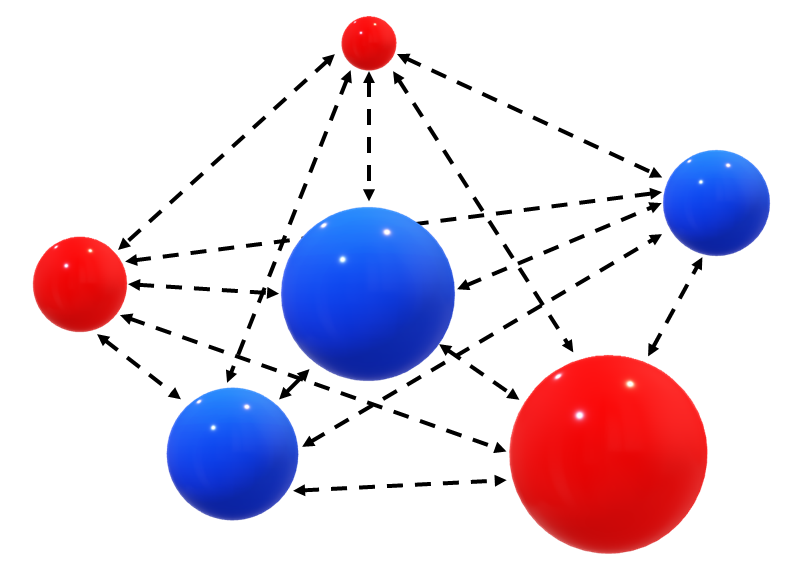
\includegraphics[width=0.35\columnwidth]{images/Nbody.png}
    \caption{Figure caption.
i}
    \label{fig:fig1}
\end{figure}

You can also include a table, like Table~\ref{table:table1}.
\begin{table}[H]%[!tb]
\centering
\footnotesize
\begin{tabular}{|p{3.9cm}|c|c|c|}
\hline
%\textbf{Distributed} proposed approach  & MOTA & MOTP & Bandwidth [kB/frame]\\
\textbf{Algorithm} & RRT & RRT* & A*\\
\hline
Computational Time (s) & 1 & 3 & 5 \\
Path distance (m)      & 5 & 3 & 1 \\
\hline
\end{tabular}
\caption{Comparison results}
\label{table:table1}
\end{table}

%%%%%%%%%%%%%%%           
% CONCLUSIONS %
%%%%%%%%%%%%%%%

\section{Conclusions}\label{sec:conclusion}
Practical work conclusions. Remember, it is part of your job to make us believe you deserve the maximum grade!!


%%%%%%%%%%%%%%           
% REFERENCES %
%%%%%%%%%%%%%%

\bibliographystyle{IEEEtran}
\bibliography{biblio}

\end{document}

